\documentclass[../main.tex]{subfiles}

\graphicspath{{../images/}}

\begin{document}
\pagestyle{fancy}
\lhead{Lecture 10: 9/26/24}
\chead{Chapter 5.5-6}
\rhead{PHYS 463}

\section{Simple Applications of macroscopic thermodynamics}

\subsection{General relationship of thermodynamics}

Fundamental thermodynamic relation for a \textit{quasi-static process}:
\begin{align*}
    dS = \frac{\dbar Q}{T}
\end{align*}
where
\begin{align*}
    \dbar Q = dE + \dbar W = dE + pdV
\end{align*}
The only external parameter of change is $V$
\begin{align*}
    \implies dE = TdS - pdV
\end{align*}
This specifies certain relationship between $T,S,p,V$ i.e. $S$ \& $V$ are independent variables
\begin{align*}
    E = E(S,V)
\end{align*}
So we have a pure mathematical relationship
\begin{align*}
    dE = \qt(\pdv{E}{S})_V dS + \qt(\pdv{E}{V})_S dV
\end{align*}
where
\begin{align*}
    \begin{cases}
        T = \qt(\pdv{E}{S})_V \\
        -p = \qt(\pdv{E}{V})_S
    \end{cases}
\end{align*}
which we already know! Because $dE$ is an exact differential
\begin{align*}
    \qt(\pdv{T}{V})_S = -\qt(\pdv{p}{S})_V
\end{align*}
this is known as the first Maxwell relation \href{https://en.wikipedia.org/wiki/Maxwell_relations#/media/File:Thermodynamic_map.svg}{(wiki)}.

\paragraph{How about} $S, P$?

From our favorite starting point
\begin{align*}
    dE = TdS - pdV 
\end{align*}
we need to change $dV \to dp$ so from chain rule
\begin{align*}
    d(pV) = p dV + V dp \implies pdV = d(pV) - V dp 
\end{align*}
so
\begin{align*}
    dE = TdS - d(pV) + V dp
\end{align*}
or
\begin{align*}
    d(E + pV) = TdS + Vdp
\end{align*}
lets call this new parameter $H = E + pV$ the \textbf{enthalpy} i.e.
\begin{align*}
    H = H(S,p)
\end{align*}
So
\begin{align*}
    \begin{cases}
        T = \qt(\pdv{H}{S})_p \\
        V = \qt(\pdv{H}{p})_S
    \end{cases}
\end{align*}
where $dH$ is an exact differential
\begin{align*}
    \qt(\pdv{T}{p})_S = \qt(\pdv{V}{S})_p
\end{align*}
or the second Maxwell relation!

\paragraph{Worksheet}
We can derive the Helmholtz free energy $F = F(T,V)$ by starting with
\begin{align*}
    d(TS) = TdS + SdT \implies TdS = d(TS) - SdT
\end{align*}
so
\begin{align*}
    dE &= d(TS) -SdT - pdV \\
    d(E - TS) &= -SdT - pdV
\end{align*}
\begin{enumerate}
    \item Thus the Hemholtz free energy $F \equiv E - TS$ so
    \begin{align*}
        dF &= dE - (TdS + SdT) \\
        &= TdS - pdV - Tds - SdT \\
        &= -SdT - pdV
    \end{align*}
    \item So $F = F(T,V)$ the we know that
    \begin{align*}
        \begin{cases}
            -S = \qt(\pdv{F}{T})_V \\
            -p = \qt(\pdv{F}{V})_T
        \end{cases}
    \end{align*}
    and $dF$ is an exact differential
    \begin{align*}
        \qt(\pdv{S}{V})_T = \qt(\pdv{p}{T})_V
    \end{align*}
\end{enumerate}
Finally for independent parameters $T,p$:
\begin{align*}
    dE = TdS - pdV 
\end{align*}
we need to change $dV \to dp$ so from chain rule
\begin{align*}
    d(pV) = p dV + V dp \implies pdV = d(pV) - V dp 
\end{align*}
so also using $TdS = d(TS) - S dT$
\begin{align*}
    dE &= (d(TS) - S dT) - (d(pV) - V dp) \\
    d(E - TS + pV) &= -S dT + V dP
\end{align*}
where $G = E - TS + pV$ is the Gibbs free energy $G = G(T,p)$
\begin{align*}
    \begin{cases}
        -S = \qt(\pdv{G}{T})_p \\
        V = \qt(\pdv{G}{p})_T
    \end{cases}
\end{align*}
and $dG$ is an exact differential
\begin{align*}
    \qt(\pdv{V}{T})_p = -\qt(\pdv{S}{p})_T
\end{align*}
\paragraph{Summary of Maxwell relations}
\begin{align*}
    \qt(\pdv{T}{V})_S &= -\qt(\pdv{p}{S})_V \\
    \qt(\pdv{T}{p})_S &= \qt(\pdv{V}{S})_p \\
    \qt(\pdv{S}{V})_T &= \qt(\pdv{p}{T})_V \\
    \qt(\pdv{V}{T})_p &= -\qt(\pdv{S}{p})_T
\end{align*}
or in box form
\begin{table}
    \centering
    \begin{tabular}{c|c}
        E & F \\ 
        \hline
        H & G
    \end{tabular}
\end{table}
Where the components are horizontal ($TS$) and vert ($pV$) give us the relations.

e.g. someothing

\newpage
\lhead{Lecture 11: 10/1/24}
\chead{Chapter 5.5-6}

\paragraph{Review of Maxwell relations} the DoS and external parameters of the system
\begin{align*}
    (T,S) \qand (p,V)
\end{align*}
are not independent, but related through
\begin{align*}
    dE = T ds - pdV
\end{align*}
From this we can get the Maxwell relations
\begin{align*}
    \qt(\pdv{T}{V})_S &= -\qt(\pdv{p}{S})_V \\
    \qt(\pdv{T}{p})_S &= \qt(\pdv{V}{S})_p \\
    \qt(\pdv{S}{V})_T &= \qt(\pdv{p}{T})_V \\
    \qt(\pdv{V}{T})_p &= -\qt(\pdv{S}{p})_T
\end{align*}
which can be derived from the Thermodynamic functions
\begin{align*}
    E &= E(S,V) \\
    H &= H(S,p) = E + pV \\
    F &= F(T,V) = E - TS \\
    G &= G(T,p) = E - TS + pV
\end{align*}

\subsection{Specific Heats}
\begin{itemize}
    \item Molar specific heat at constant volume $dV = 0$
    \begin{align*}
        C_V = \frac{1}{n} \qt(\frac{\dbar Q}{dT})_V \quad dE = \dbar Q = n C_v dT
    \end{align*}
    \item Molar specific heat for constant pressure $dp = 0$
    \begin{align*}
        C_p = \frac{1}{n} \qt(\frac{\dbar Q}{dT})_p = C_V + \frac{1}{n} p \qt(\frac{dV}{dT})_p
    \end{align*}
    When comparing the two specific heats we can infer that $C_p > C_V$ because the heat $\dbar Q$ has to both increase the internal energy and do mechanical work to expand the volume:
    \begin{align*}
        \dbar Q = dE + pdV = n C_V dT + pdV
    \end{align*}
    \item For an ideal gas
    \begin{align*}
        pV &= nRT \\
        p dV &= nR dT \\
        \implies \qt(\frac{dV}{dT}) &= \frac{nR}{p}
    \end{align*}
    thus
    \begin{align*}
        C_p = C_V + R
    \end{align*}
    where we define
    \begin{align*}
        \gamma = \frac{C_p}{C_v} = 1 + \frac{R}{C_V}
    \end{align*}
\end{itemize}
For the idea gas molecule the energy is given by
\begin{align*}
    E(T) = \frac{3}{2} nRT 
\end{align*}
where there is $3$ degrees of freedom thus
\begin{align*}
    C_V &=  \frac{1}{n} \frac{dE}{dT} = \frac{3}{2} R \\
    C_p &= C_V + R = \frac{5}{2} R
\end{align*}
For a diatomimc molecule there are 2 extra degrees of freedom for rotaion so
\begin{align*}
    \gamma = \frac{C_p}{C_V} = \frac{5}{3}
\end{align*}

\subsection{Adiabatic expansion or compression}

Some definitions:
\begin{itemize}
    \item ``Isothermal'': $T$ is constant $\implies pV =$ Constant.
    \item ``Adiabatic'': $\dbar Q = 0$ 
    \begin{align*}
        \implies 0 &= dE + pdV \\
        &= n C_V dT + pdV
    \end{align*}
\end{itemize}
So from the ideal gas law $pV = nRT$ we can get
\begin{align*}
    V dP + pdV = nR dT
\end{align*}
and substituting $dT$ into the adiabatic expression
\begin{align*}
    \dbar Q = 0 = V \frac{C_V}{R} dP + \frac{C_V P}{R} dV + p dV
\end{align*}
which can be rewritten as
\begin{align*}
    0 = (C_V + R) pdV + C_V V dP = C_p pdV + C_v V dp
\end{align*}
or dividing by $C_V PV$ we ge
\begin{align*}
    \gamma \frac{dV}{V} + \frac{dP}{P} = 0
\end{align*} 
Integration then gives
\begin{align*}
    \gamma \ln V + \ln P = \textrm{Constant} \implies \ln (PV^\gamma) = \textrm{Constant}
\end{align*}
or 
\begin{align*}
    PV^\gamma = \textrm{Constant}
\end{align*}

\paragraph{Worksheet}
\begin{itemize}
    \item Pumping a bike tire, a liter or air at 1 atm is compressed \textit{adiabatically} to 7 atm. (Air is mostly diatomic gas)
    \begin{itemize}
        \item For diatomic gas
        \begin{align*}
            E(T) = \frac{5}{2} nRT
        \end{align*}
        So the specific heats are
        \begin{align*}
            C_V = \frac{1}{n} \frac{dE}{dT} = \frac{5}{2} R
            C_p = C_V + R = \frac{7}{2} R
        \end{align*}
        which gives us
        \begin{align*}
            \gamma = \frac{C_p}{C_V} = \frac{7}{5}
        \end{align*}
        \item The final volume after compression is
        \begin{align*}
            p_i V_i^\gamma = p_f V_f^\gamma
        \end{align*}
        or
        \begin{align*}
            (\qty{1}{atm}) (\qty{1}{L})^{7/5} = (\qty{7}{atm}) V_f^{7/5} \implies V_f = \qty{0.25}{L}
        \end{align*}
        \item Work done compressing air: using $p_i V_i^\gamma = 1 \implies p = \frac{1}{V^\gamma}$
        \begin{align*}
            W = \int_{V_i}^{V_f} p dV &= \int_{V_i}^{V_f} \frac{1}{V^\gamma} dV \\
            &= \frac{1}{1-\gamma} \qt(V_f^{1-\gamma} - V_i^{1-\gamma}) \\
        \end{align*}
        \item If initial temp is $300$ K, the final temp is
        \begin{align*}
            P_i V_i &= nR T_i \quad P_f V_f = nR T_f \\
            &\implies \frac{P_f V_f}{P_i V_i} = \frac{T_f}{T_i}
        \end{align*}
    \end{itemize}
    \item If the compression is isothermal (pumping very slowly) how does the answers change?
\end{itemize}

\paragraph{General case:}
\begin{align*}
    C_V &= \qt(\frac{\dbar Q}{dT})_V = T (\pdv{S}{T})_V \\
    C_p &= \qt(\frac{\dbar Q}{dT})_p = T (\pdv{S}{T})_p
\end{align*}

\subsection{Entropy}
Consider $S = S(T,P)$
\begin{align*}
    \dbar Q = T dS &= T\qt[
        \qt(\pdv{s}{T})_P dT + \qt(\pdv{S}{P})_T dP
    ] \\
    &= C_P dT + T \qt(\pdv{S}{P})_T dP
\end{align*}

\newpage
\lhead{Lecture 12: 10/3/24}
\chead{Chapter 5.7-5.9}
\subsection{Specifc heats again}

General relation between $C_v$ and $C_p$ for non-ideal gas ($C_p - C_v = R$), 
\begin{align*}
    C_V = \qt(\frac{\dbar Q}{dT})_V = T \qt(\pdv{S}{T})_V \\
    C_P = \qt(\frac{\dbar Q}{dT})_P = T \qt(\pdv{S}{T})_P
\end{align*}
where
\begin{align*}
    \dbar Q = T dS &= T \qt[
        \qt(\pdv{S}{T})_P dT + \qt(\pdv{S}{P})_T dP
    ] \\
    &= C_P dT + T \qt(\pdv{S}{P})_T dP
\end{align*}
The pressure $P(T,V)$ with temp and volume dependence has a differential
\begin{align*}
    dP = \qt(\pdv{P}{T})_V dT + \qt(\pdv{P}{V})_T dV
\end{align*}
and since $C_V$ acknowledges fixed volume $dV = 0$ we get
\begin{align*}
    C_V = \qt(\frac{\dbar Q}{dT})_V = C_p + T \qt(\pdv{S}{p})_T \qt(\pdv{P}{T})_V 
\end{align*}
where we can replace the entropy term wit the Maxwell relation
\begin{align*}
    \qt(\pdv{S}{P})_T = -\qt(\pdv{V}{T})_P
\end{align*}
We define the ``volume coefficient of expansion''
\begin{align*}
    \alpha \equiv \frac{1}{V} \qt(\pdv{V}{T})_P
\end{align*}
so
\begin{align*}
    \qt(\pdv{S}{P})_T = - \alpha V
\end{align*}
The second term is not well defined since fixing volume while increasing pressure is hard to due (e.g. filling a water bottle with more and more water). 
Now using the volume dependence $V(P,T)$ i.e.
\begin{align*}
    dV = \qt(\pdv{V}{T})_P dT + \qt(\pdv{V}{P})_T dP = 0
\end{align*}
and moving thing around we get
\begin{align*}
    \qt(\frac{dP}{dT})_V = - \frac{\qt(\pdv{V}{T})_P}{\qt(\pdv{V}{P})_T}
\end{align*}
where we define another term
\begin{align*}
    \kappa = -\frac{1}{V} \qt(\pdv{V}{P})_T
\end{align*}
AKA the ``isothermal compressibility'' thus
\begin{align*}
    \boxed{C_P - C_V = VT \frac{\alpha^2}{\kappa}} 
\end{align*}
One check we can do is use the Ideal gas law to calculate $\alpha$ and $\kappa$ then see if the above equation gives us the relation $C_P - C_V = R$

\subsection{Entropy and Internala energy}

$S(T,V)$ doing the same thing
\begin{align*}
    dS &= \qt(\pdv{S}{T})_V dT + \qt(\pdv{S}{V})_T dV \\
    &= \frac{C_V}{T} dT + \qt(\pdv{P}{T})_N dV
\end{align*}
etc.

\subsection{Free expansion of a gas} 

For the general case
\begin{gather*}
    dE = 0 \\
    E = E(T,V)
\end{gather*}

% fig5_1.png
\begin{figure*}[ht]
    \centering
    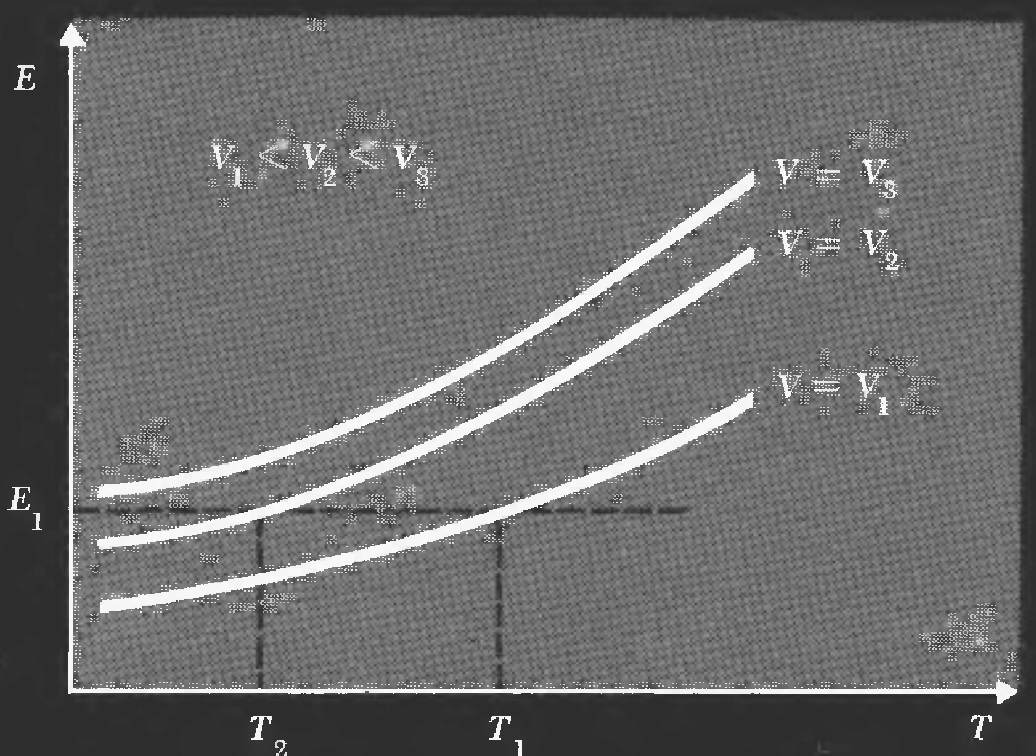
\includegraphics[width=0.5\textwidth]{fig5_1.png}
    \caption{Free expansion of a gas}
    \label{fig:5_1}
\end{figure*}

\paragraph{Van de Waals Gas}
\begin{gather*}
    \qt(P + \frac{a}{v^2}) (v - b) = RT \quad E = E(T,V) \\
    v = \frac{V}{n}
\end{gather*}

\newpage
\chead{Chapter 5.11}
\subsection{Heat Engine}
What is a heat engine? Heat $\to$ Work.

% fig5_2.png Heat Engine diagrams
\begin{figure*}[ht]
    \centering
    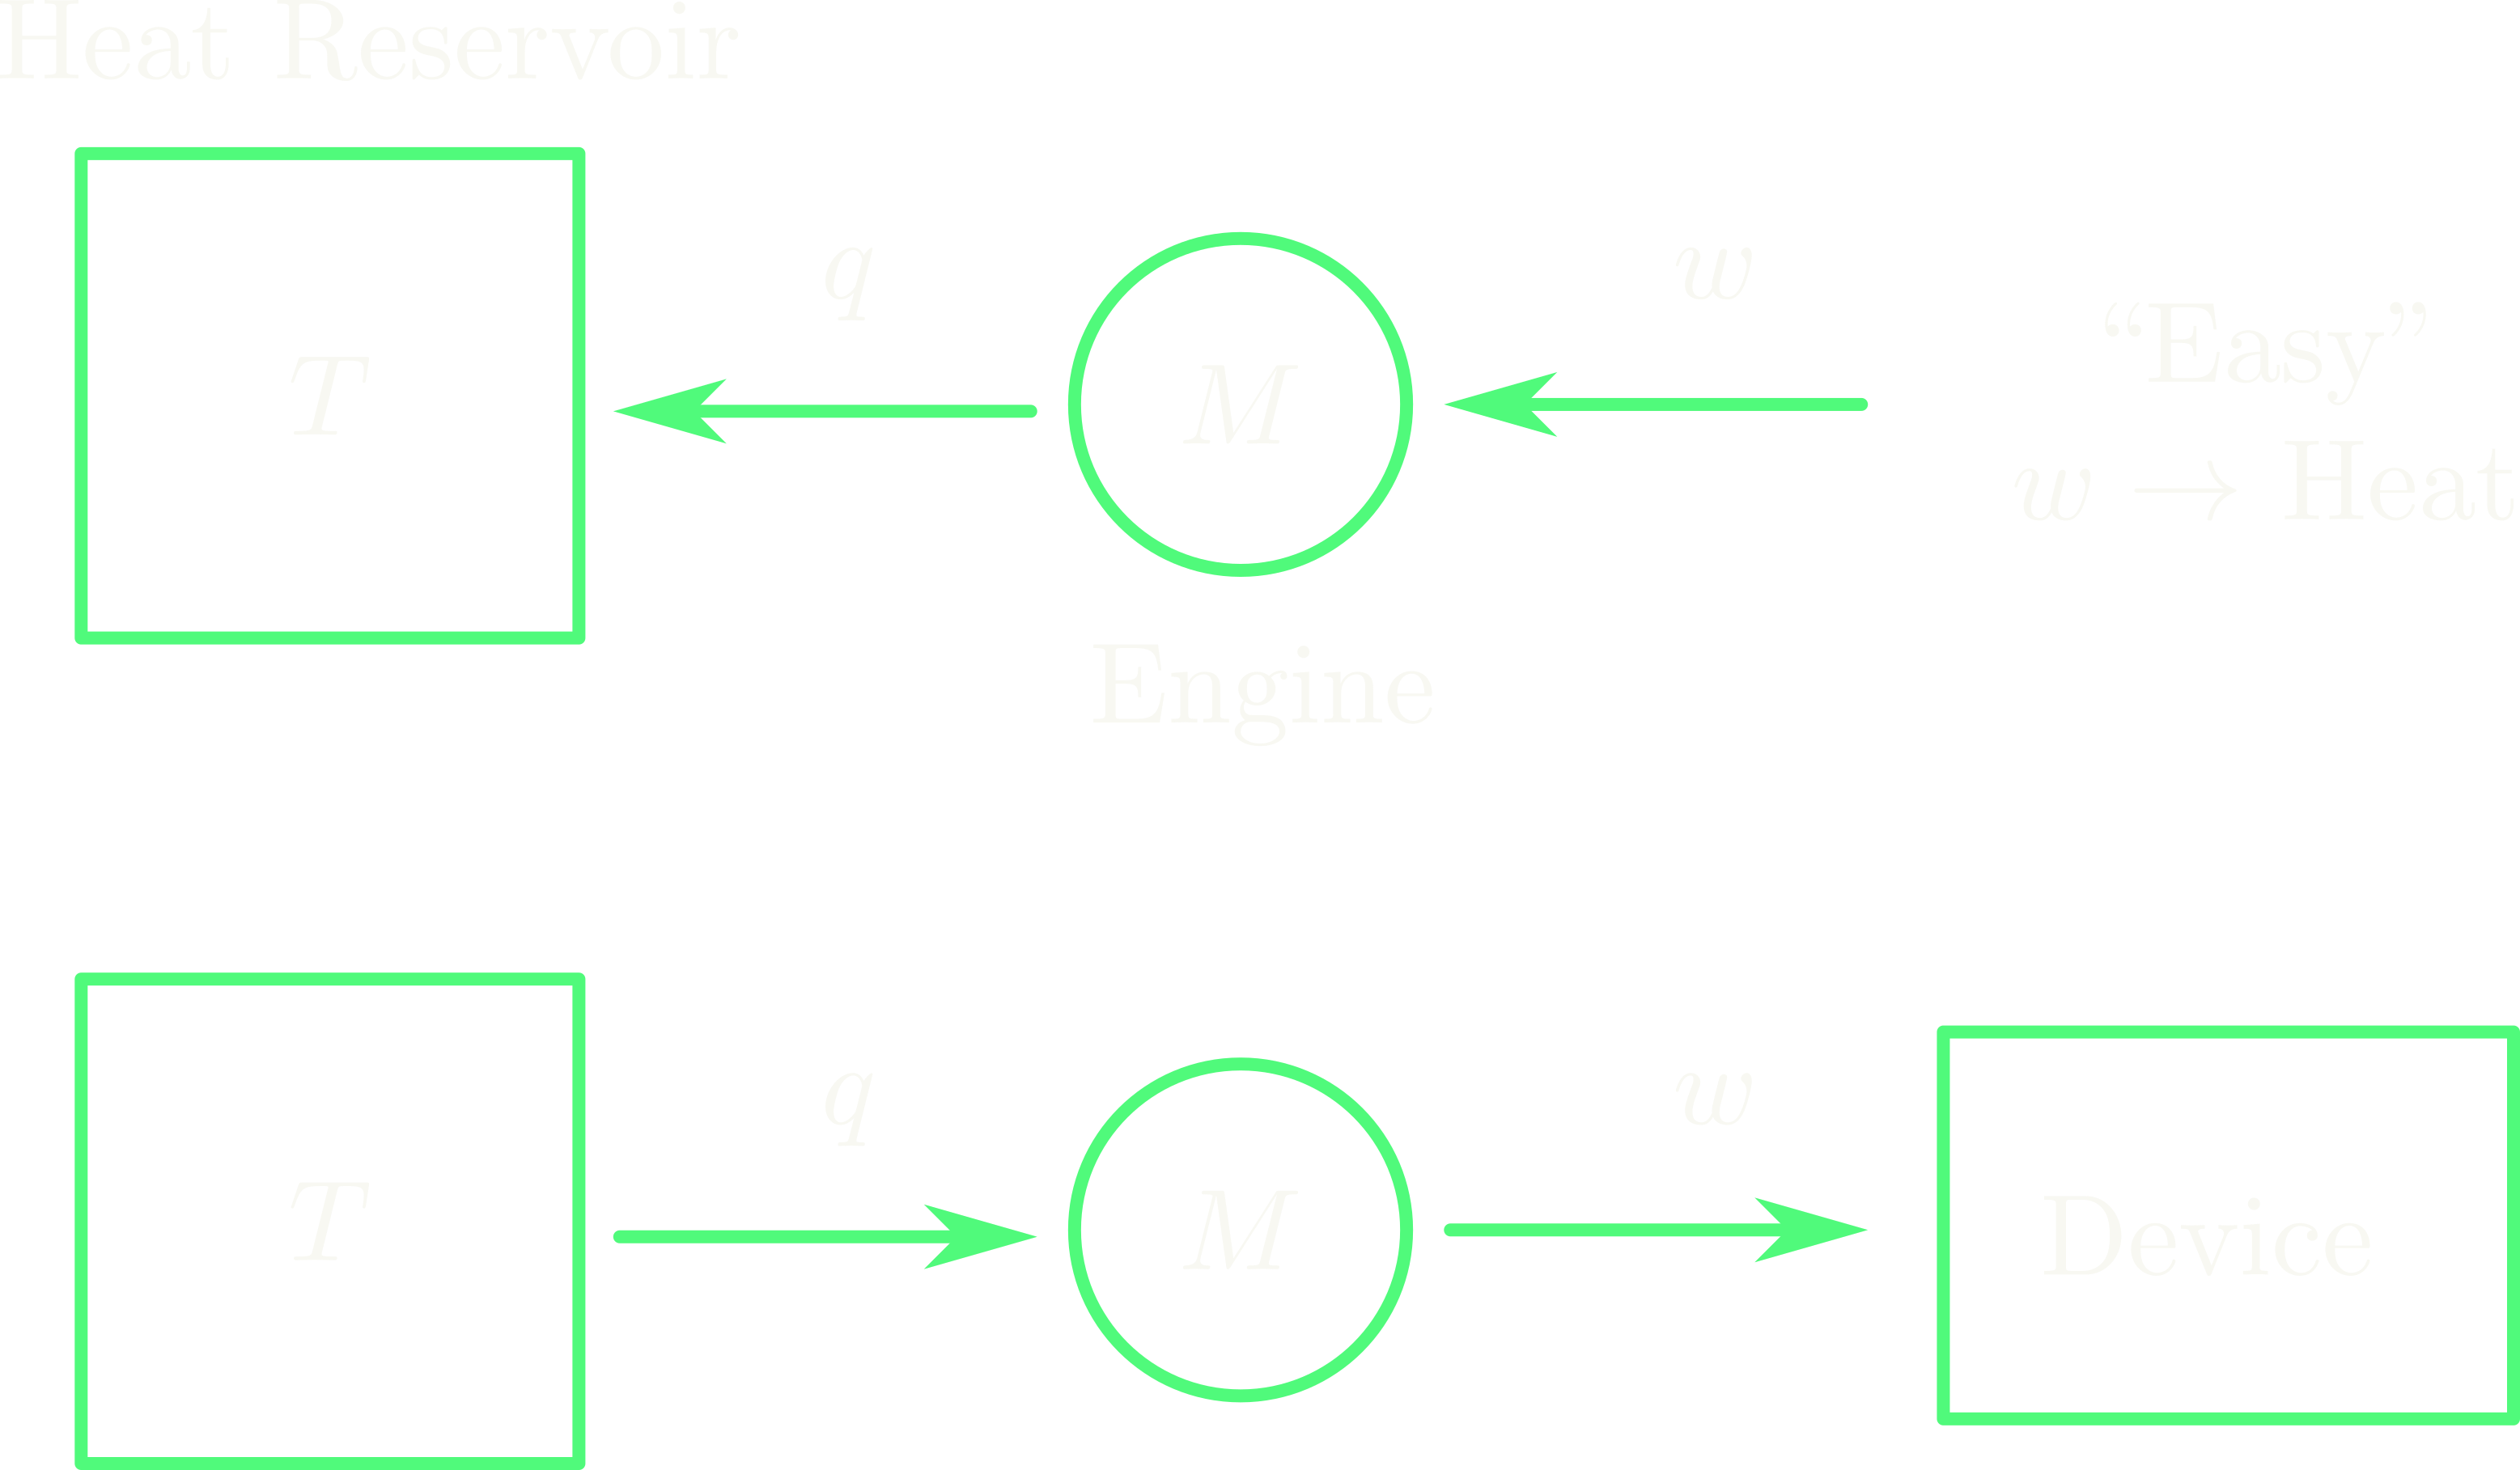
\includegraphics[width=0.5\textwidth]{fig5_2.png}
    \captionsetup{width=0.8\textwidth}
    \caption{(top) reverse ``easy'' process converting work to heat. (botton) Heat Engine converting heat from a reservoir into work.}
    \label{fig:5_2}
\end{figure*}

\begin{itemize}
    \item For a heat engine: whatever mechanisms needed to retune to the same 
    original condition; go through a cycle; otherwise, engine cannot continuously operate.
    \item Ideally perfect engine: $q = w$ or $100\%$ efficiency
\end{itemize}

A perfect engine \textit{violates} the 2nd law of thermodynamics $\Delta S \geq 0$.
\begin{itemize}
    \item entropy change for engine and external device $\Delta S = 0$
    \item entropy change for hea reservoir $\Delta S = -q/T$ thus
    \begin{align*}
        \Delta S_\text{tot} = -\frac{q}{T} < 0
    \end{align*}
\end{itemize}

Building a heat engine: Using two heat reservoirs

\begin{figure*}[ht]
    \centering
    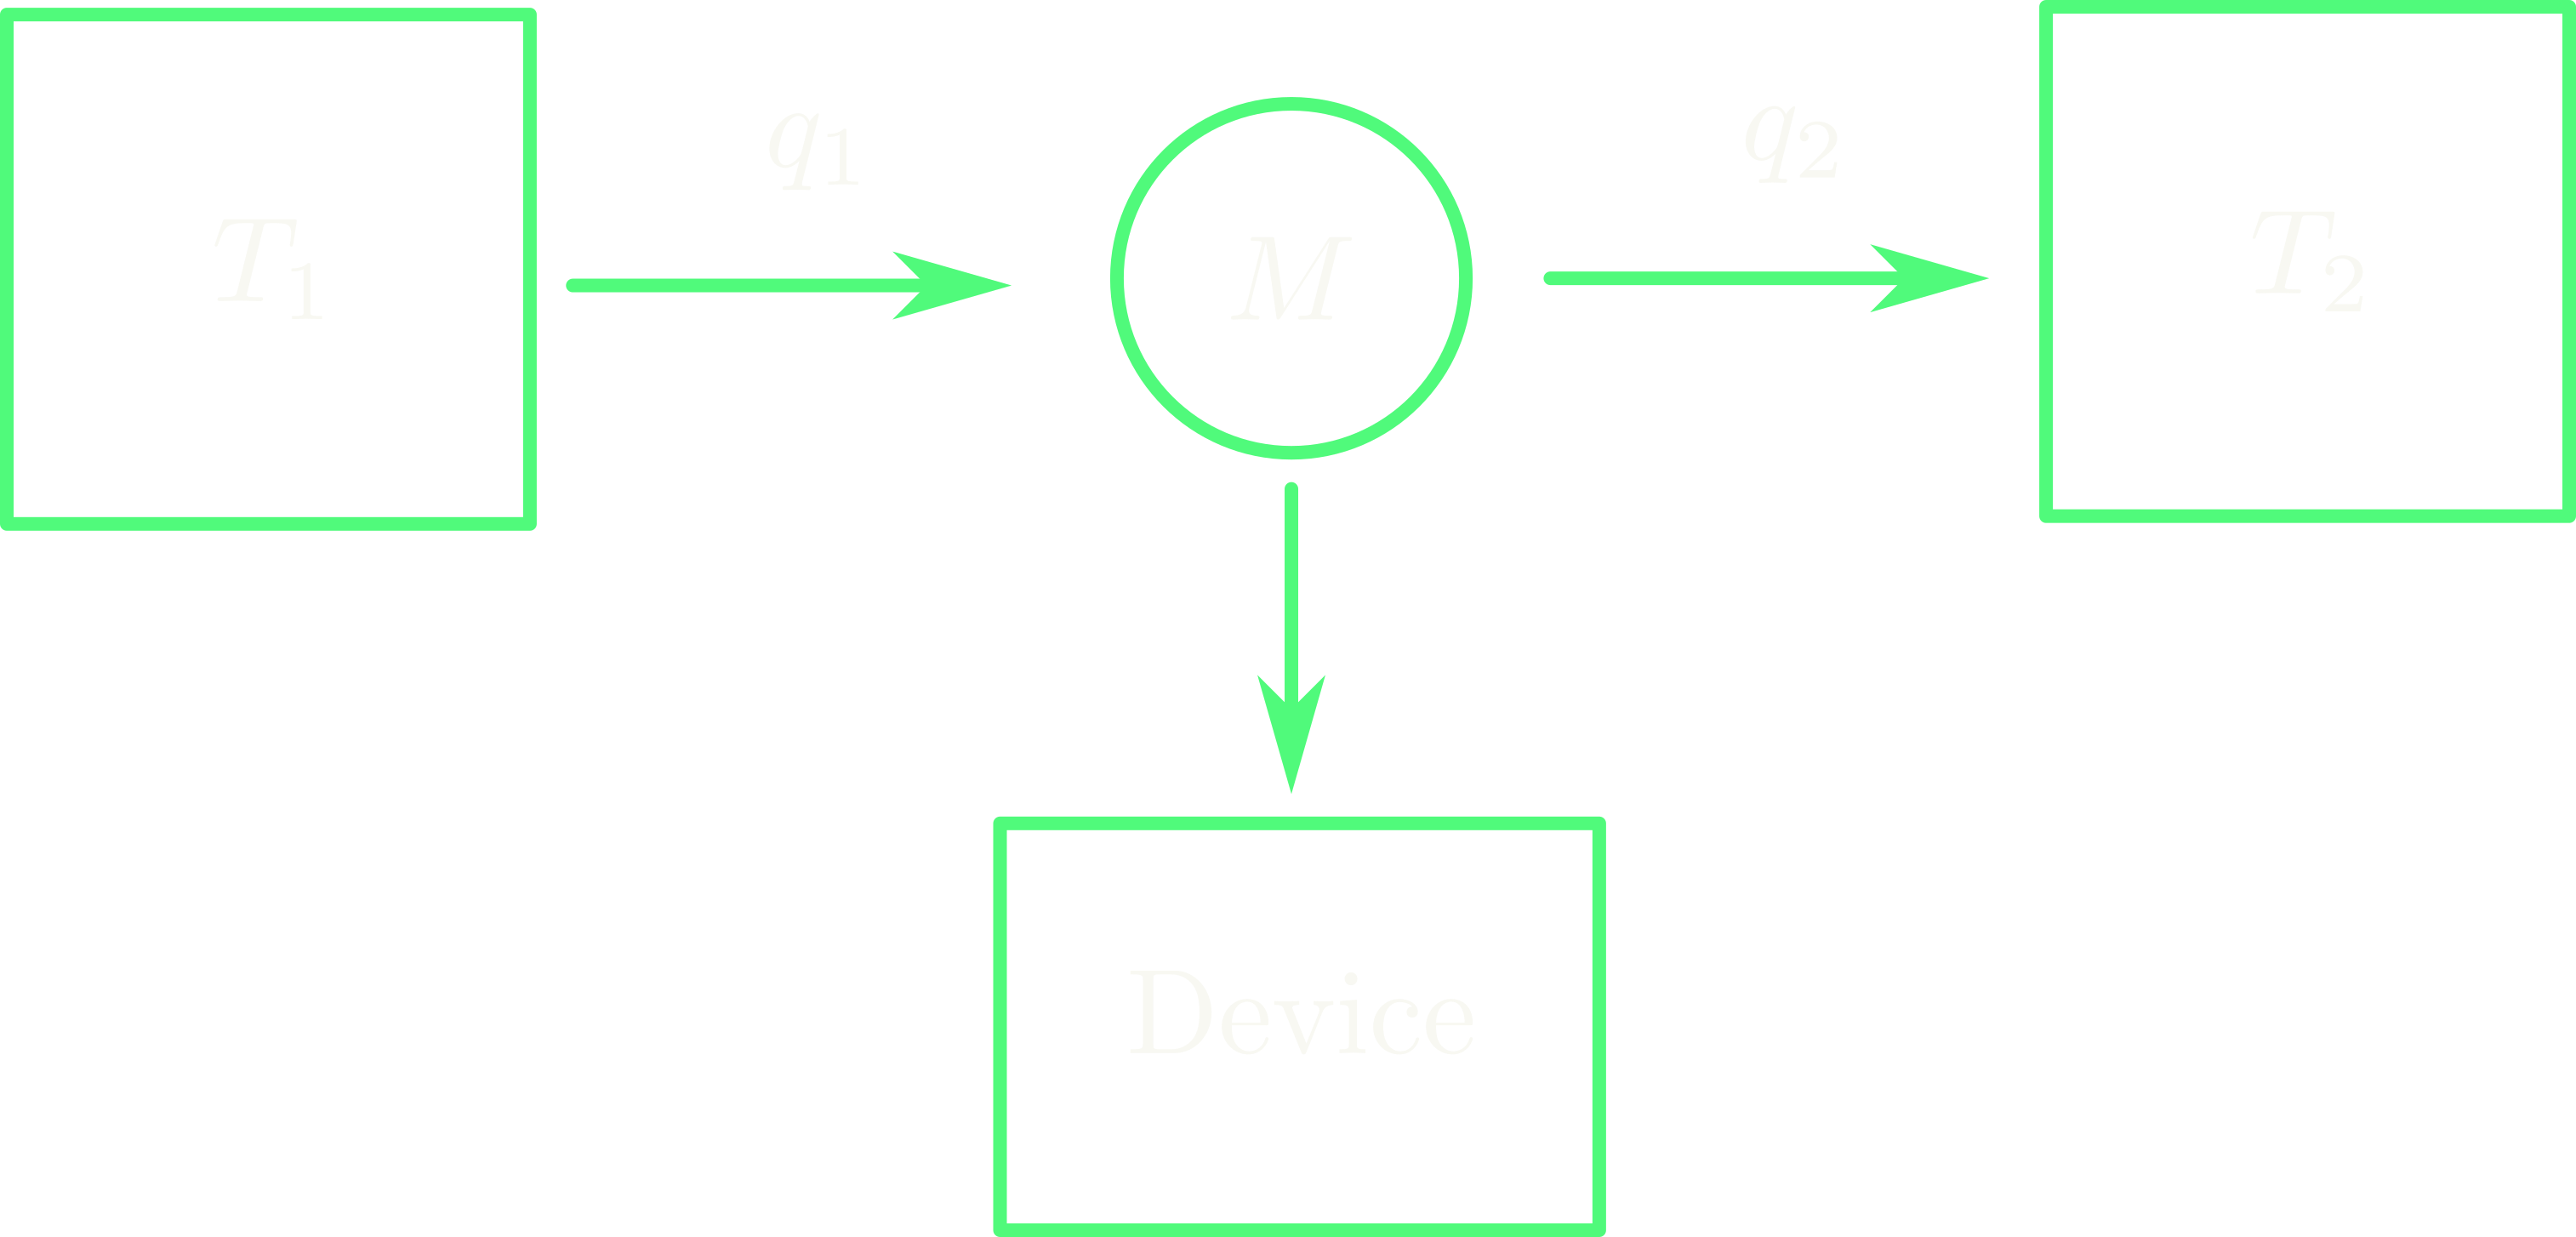
\includegraphics[width=0.5\textwidth]{fig5_3.png}
    \caption{Heat engine using two heat reservoirs}
    \label{fig:5_3}
\end{figure*}

Where we make $q_1 > q_2$ so that heat flows from $T_1 \to T_2$ so that
\begin{align*}
    W = q_1 - q_2 \implies q_2 = q_1 - W
\end{align*}
so the total entropy change is
\begin{align*}
    \Delta S_\text{tot} &= -\frac{q_1}{T_1} - \frac{q_2}{T_2} \geq 0 \\
    &= -\frac{q_1}{T_1} + \frac{q_1 - W}{T_2} \\
    \implies \frac{W}{T_2} &\leq q_1 \qt(\frac{1}{T_1} - \frac{1}{T_2})
\end{align*}
thus the efficiency of the engine
\begin{align*}
    \eta = \frac{W}{q_1} &\leq  T_2 \qt(\frac{1}{T_2} - \frac{1}{T_1}) \\
    &= 1 - \frac{T_2}{T_1}
\end{align*}

\subsubsection*{Carnot Engine} 

\begin{figure*}[ht]
    \centering
    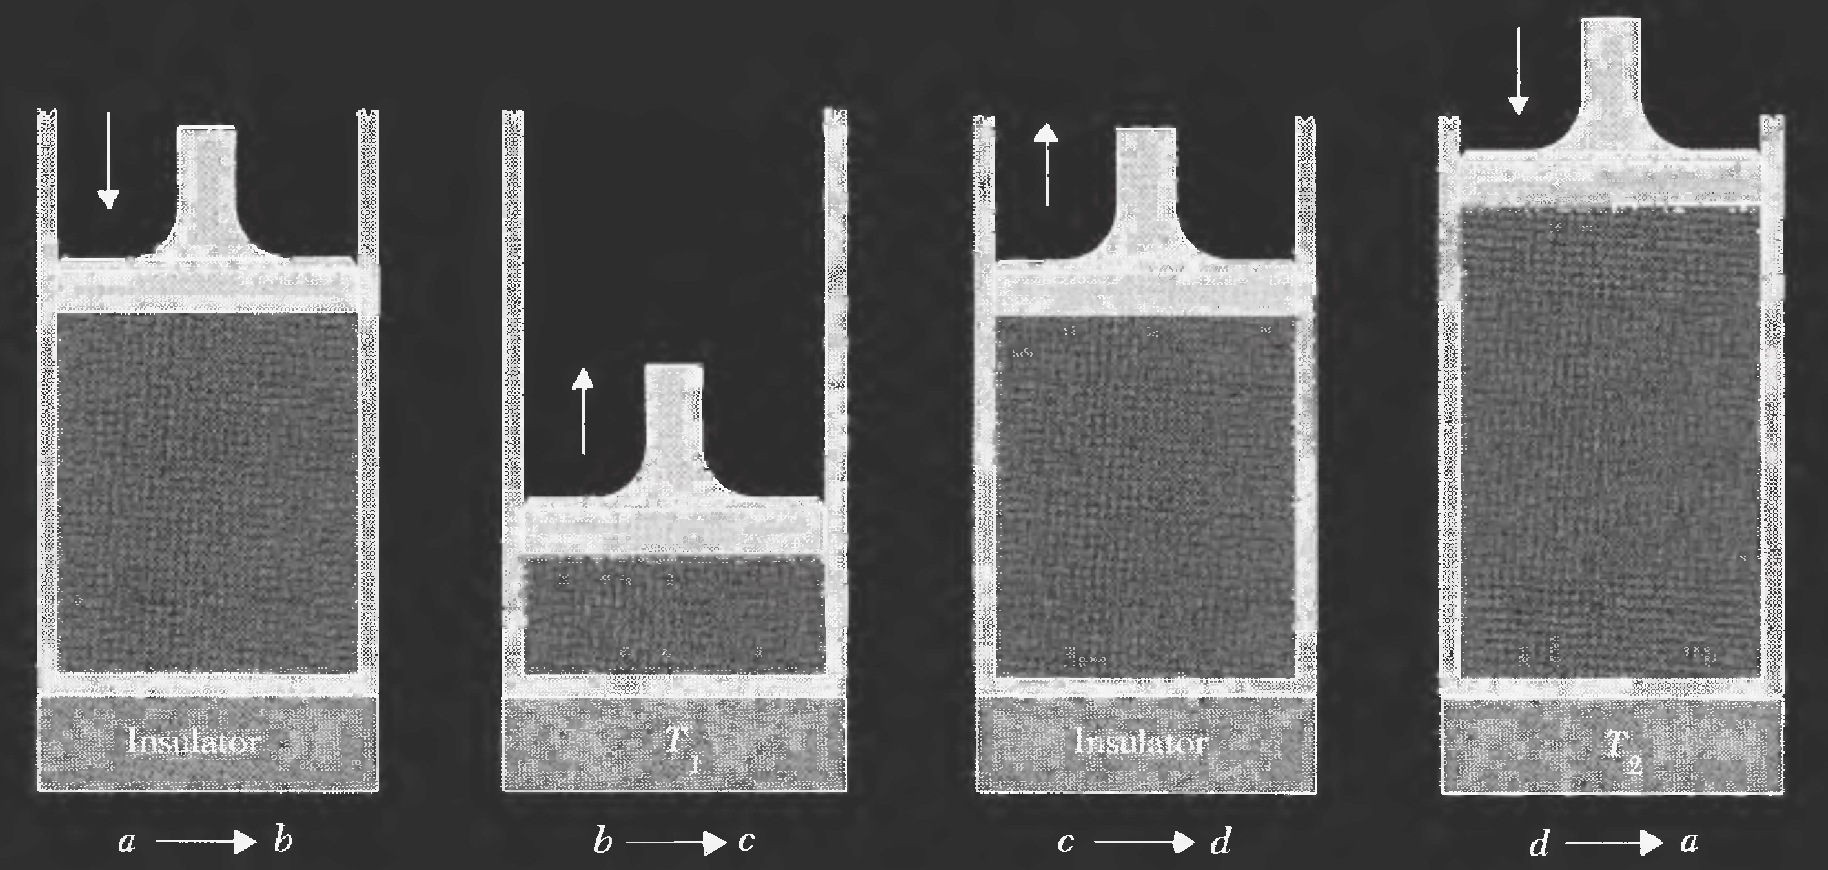
\includegraphics[width=0.5\textwidth]{fig5_4.png}
    \caption{4 stages of Carnot Engine}
    \label{fig:5_4}
\end{figure*}

\begin{itemize}
    \item $a \to b$: adiabatic (no heat exchange) bringing colder $T_2 \to T_1$
    \item $b \to c$: isothermal (constant temp) adding heat $q_1$ from hot reservoir
    \item $c \to d$: adiabatic (no heat exchange) cooling down $T_1 \to T_2$ as work is done through expansion
    \item $d \to a$: isothermal (constant temp) releasing heat $q_2$ to cold reservoir
\end{itemize}

\paragraph{Worksheet} Carnot Engine using an ideal gas:

The work done is
\begin{align*}
    W = \int_a^b PdV + \int_b^c PdV + \int_c^d PdV + \int_d^a PdV
\end{align*}
so using the ideal gas law $PV = nRT$
\end{document} 

